\section{Выполнение работы}
\subsection{Описание тестового стенда}
Для выполнения работы использовалось два тестовых стенда:
\begin{itemize}
\item Платформа Raspberry Pi 1 с ОС ArchLinux
\item Виртуальная машина с Arch Linux
\end{itemize}

Благодаря тому, что платформы Raspberry Pi 1 и Raspberry Pi Zero аппаратно полностью совместимы, ОМ разработанный на платформе RPi 1 будет совместим с RPi Zero. Однако, проблема в том, что RPi имеет проприетарную графику, которая не поддерживается в Wayland. Поэтому, задача конфигурирования ОС на платформе RPi включала в себя установку драйвера VC4~\cite{vc4}, который позволяет представить видеокарту RPi как стандартное DRI устройство.

Виртуальная машина c ArchLinux была установлена в гипервизоре VirtualBox. Однако, из-за того что в VirtualBox не реализована поддержка протокла Wayland, мобильный оконный менеджер запускался в качестве X-клиента в оконном менеджере xfce4.

\subsection{Выбор библиотеки-композитора}
Как было сказано ранее, в архитектуре Wayland оконный менеджер обязательно должен включать в себя композитор (в отличие от X). Так как реализация собственного Wayland-композитора с нуля --- задача слишком объемная и трудоемкая, был решено использовать какую-либо библиотеку-композитор. В таком случае задачей разработанного ОМ будет управление окнами.

Из проанализированных библиотек было решено выбрать библиотеку wlc по нескольким причинам:
\begin{itemize}
\item API библиотеки устойчив и проверен
\item на ее основе уже реализовано некоторое количество программ
\item для библиотеки есть некоторое количество примеров
\end{itemize}

\subsection{Разработка оконного менеджера}
Исходный код основного файла оконного менеджера приведен в листинге~\ref{lst:main}. В основной функции приложения main производятся следующие действия:
\begin{itemize}
\item анализируются аргументы командной строки (строки 358-365)
\item считывается конфигурация (строка 367)
\item устанавливаются функции-обработчики действий для wlc (строки 370-392)
\item инициализируется композитор (строки 395-397)
\item запускаются системные приложения (строка состояния и рабочий стол) (строки 399-425)
\item запускается оконный менеджер (строка 426)
\end{itemize}

Созданное приложение принимает один аргумент --- файл конфигурации. Если аргумент не указан, ищется и открывается файл по-умолчанию -- \texttt{~/.config/xxwm}. Пример конфигурационного файла приведен в листинге \ref{lst:conf}. В нем указываются пути к исполняемым файлам строки состояния и рабочего стола.

\begin{lstlisting}[label=lst:conf, caption={Формат конфигурационного файла ОМ}]
[statusbar]
exe=/home/kivi/workspace/Phone/src/status_bar/status

[desktop]
exe=/home/kivi/workspace/Phone/src/desktop/desktop
\end{lstlisting}

Считывание конфигурационного файла производится с помощью библиотеки inih. Исходные коды функций, которые производят считывание конфигурационного файла приведены в листингах \ref{lst:confh} -- \ref{lst:confc}.

Далее в функции main устанавливаются функции-обработчики для библиотеки-композитора. Данные функции обрабатывают события, получаемые от композитора и, соответственно, работают с типами данных композитора.  Композитор определяет несколько абстракций:
\begin{itemize}
\item output --- вся область отображения на экран. В терминах оконных менеджеров это соответствует "рабочему столу"
\item view --- окно приложения
\end{itemize}

Рассмотрим все эти функции более подробно.
\begin{itemize}
\item \texttt{wlc\_log\_set\_handler} устанавливает функцию, которая будет осуществлять логирование. В нашем случае устанавливается функция, которая просто выводит все сообщения в терминал с использованием функции \texttt{printf} (строчки 352-355).

\item \texttt{wlc\_set\_output\_resolution\_cb} устанавливает функцию, которая обрабатывает изменение разрешения экрана. Устанавливаемая функция \texttt{output\_resolution} просто вызывает функцию перерисовки окон \texttt{relayout} (строчки 174-177).

\item \texttt{wlc\_set\_view\_created\_cb} устанавливает функцию, которая будет вызываться при создании нового окна. Устанавливаемая функция \texttt{view\_created} устанавливает окну необходимые флаги, выносит окно на первый план, переключает фокус на это окно и вызывает функцию перерисовки (строки 180-192).

\item \texttt{wlc\_set\_view\_destroyed\_cb} устанавливает функцию, которая будет вызваться при уничтожении окна. Устанавливаемая функция \texttt{view\_destroyed} устанавливает фокус на самое верхнее окно и вызывает функцию перерисовки (строки 195-200).

\item \texttt{wlc\_set\_view\_focus\_cb} устанавливает функцию, которая отвечает за установку фокуса на окно. Устанавливаемая функция \texttt{view\_focus} устанавливает окну флаг \texttt{WLC\_BIT\_ACTIATED} (строчки 203-206).

\item \texttt{wlc\_set\_view\_request\_move\_cb} устанавливает функцию, которая отвечает за перемещение какого-либо окна по экрану. Устанавливаемая функция \texttt{view\_request\_move} вызывает функцию \texttt{start\_interactive\_move} (строчка 210), которая в свою очередь начинает интерактивное действие вызвав функцию \texttt{start\_interactive\_action} (строчка 42).  Функция \texttt{start\_interactive\_action} сохраняет параметры окна, на котором начато интерактивное действие, в глобальную переменную и выводит это окно на первый план (строчки 26-38).

\item \texttt{wlc\_set\_view\_request\_resize\_cb} устанавливает функцию, которая отвечает за изменение размеров окна. Устанавливаемая функция \texttt{view\_request\_resize} начинает интерактивное действие изменения окна вызывая функцию \texttt{start\_interactive\_resize} (строчка 215). Данная функция начинает интерактивное действие вызвав функцию \texttt{start\_interactive\_action}, а затем определяет то, какую грань окна необходимо перемещать (строчки 46-66). Так же данная функция устанавливает окну флаг \texttt{WLC\_BIT\_RESIZING}, который указывает на то, что окно в текущий момент меняет свой размер.

\item \texttt{wlc\_set\_view\_request\_geometry\_cb} устанавливает функцию, которая отвечает за установку указанному окну определенных размеров. Устанавливаемая функция \texttt{view\_request\_geometry} не делает ничего, так как ОМ не предполагает возможности изменять размер окна извне.

\item \texttt{wlc\_set\_keyboard\_key\_cb} устанавливает функцию-обработчик нажатий клавиатуры. Устанавливаемая функция \texttt{keyboard\_key} считывает код нажатой клавиши, флаги модификаторов (CTRL, ALT и т.д.) и обрабатывает следующие комбинации (строчки 225-266):
\begin{itemize}
\item CTRL+q --- закрытие активного окна (если это не системное приложение)
\item CTRL+стрелка вниз --- переключиться на следующее окно (аналог ALT+Tab в Windows)
\item CTRL+Escape --- завершить работу оконного менеджера
\item CTRL+Enter --- запустить терминал
\end{itemize}

\item \texttt{wlc\_set\_pointer\_button\_cb} устанавливает функцию-обработчик нажатий кнопок мыши. Устанавливаемая функция \texttt{pointer\_button} обрабатывает следующие комбинации (строчки 268-291):
\begin{itemize}
\item CTRL+ЛКМ --- переместить окно
\item CTRL+ПКМ --- изменить размеры окна
\end{itemize}

\item \texttt{wlc\_set\_pointer\_motion\_cb} устанавливает функцию-обработчик передвижения мыши. Устанавливаемая функция \texttt{pointer\_motion} проверяет, если в данный момент выполняется интерактивное действие, она соответствующим образом изменяет отображение активного окна (передвигает или изменяет размеры, в зависимости от выполняемого действия) (строчки 294-350).
\end{itemize}

Далее в функции main выполняется запуск системных приложений (строки состояния и рабочего стола) и запуск самого композитора. При этом, ОМ запоминает PID системных приложений для возможности их идентификации. Например, на основе этих PID ОМ решает можно ли закрывать соответствующее окно.

Одной из самых главных функций ОМ является функция перерисовки окно \texttt{relayout} (строки 90-171). Данная функция действует по следующему алгоритму:
\begin{enumerate}
\item берет самое верхнее (переднее) окно
\item проверяем, является ли окно окном строки состояния
\item если да, то запоминаем идентификатор окна
\item если нет, то рисуем данное окно на весь экран, кроме верхней строчки высотой в 30 пикселей
\item обновляем окно строки состояния перерисовывая ее в верхних 30 пикселях экрана 
\end{enumerate}

Данный алгоритм позволяет каждый раз перерисовывать максимум два окно: активное окно приложения и окно строки состояния. Строку состояние необходимо перерисовывать, потому что в какой-то момент времени могло изменится разрешение экрана. Данный алгоритм позволяет снизить вычислительную нагрузку ОМ на систему. 

Так же при перерисовке окна учитываются флаги типа окна. Библиотека WLC определяет пять флагов окна. Экспериментальным путем было выяснено, что при работе ОМ появляются и должны по-особому отображаться только два типа окон:
\begin{itemize}
\item \texttt{WLC\_BIT\_UNMANAGED} --- окна меню
\item \texttt{WLC\_BIT\_POPUP} --- уведомления и контекстные меню (вызываемые при нажатии ПКМ)
\end{itemize}

Данные типы окон отображаются по-особому. Окна меню отображаются в соответствии с изначально заданными им параметрами, ничего не изменяется. Окна контекстных меню смещаются относительно координат их окна-родителя и координат нажатия мыши. Остальные окна отображаются по-умолчанию на всю область экрана, незанятую строкой состояния.

Примеры работы оконного менеджера приведены на рисунках \ref{fig:wm1} -- \ref{fig:wm4}.
\begin{figure}[h!]
\center{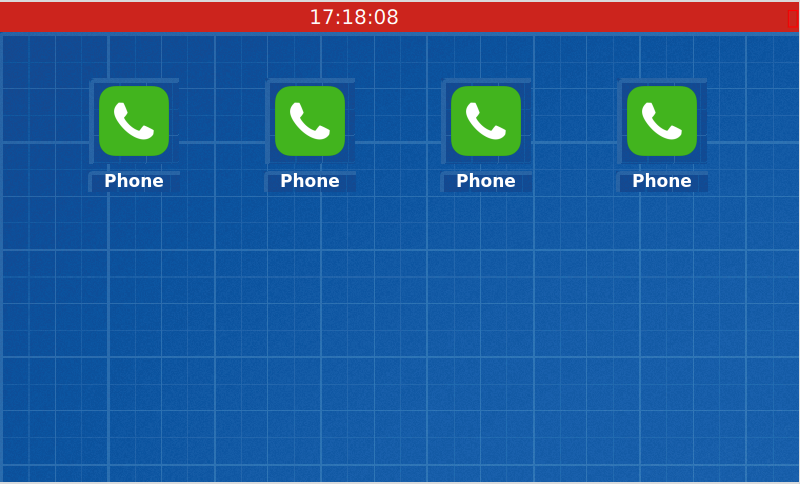
\includegraphics[width=\linewidth]{wm1}}
\caption{Оконный менеджер}
\label{fig:wm1}
\end{figure}
\begin{figure}[h!]
\center{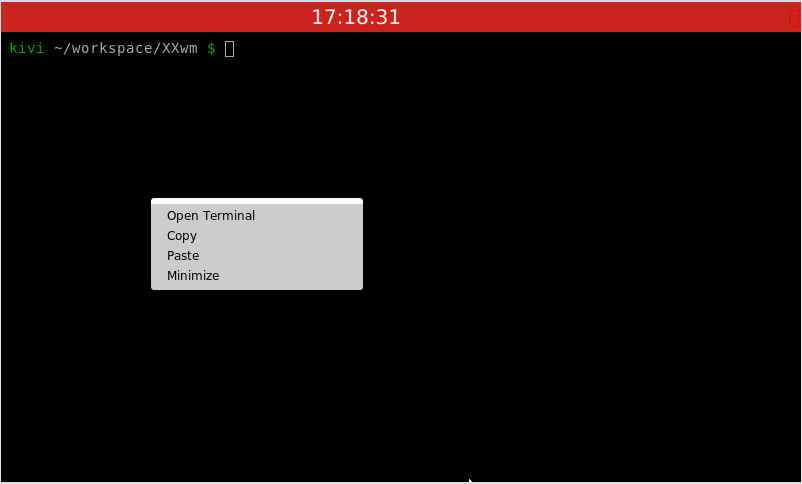
\includegraphics[width=\linewidth]{wm2}}
\caption{Отображение терминала и контекстного меню}
\label{fig:wm2}
\end{figure}
\begin{figure}[h!]
\center{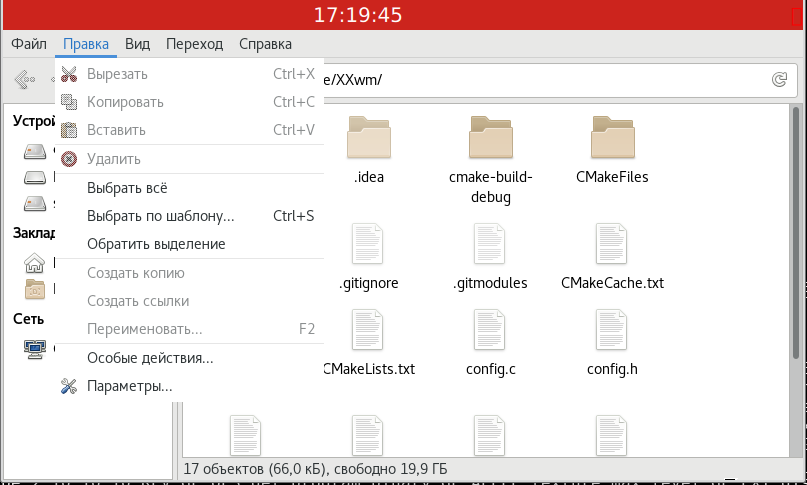
\includegraphics[width=\linewidth]{wm3}}
\caption{Отображение файлового менеджера и меню}
\label{fig:wm3}
\end{figure}
\begin{figure}[h!]
\center{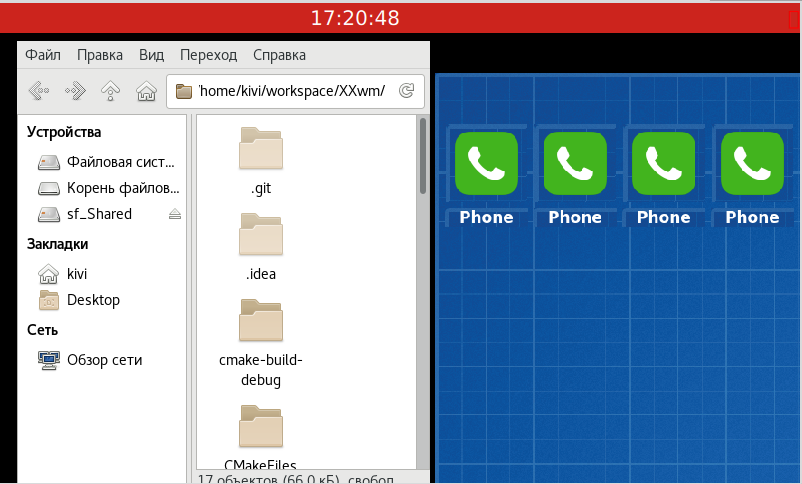
\includegraphics[width=\linewidth]{wm4}}
\caption{Перемещение и изменение размеров окон}
\label{fig:wm4}
\end{figure}

\subsection{Добавление ОМ в экранный менеджер}
Экранный менеджер или менеджер входа --- графический экран, который отображается в конце процесса загрузки вместо стандартного приглашения командной строки. Экранный менеджер представляет собой экран ввода имени пользователя и пароля для входа в систему. Существует большое количество экранных менеджеров, однако все они детектируют установленные в систему оконные менеджеры по конфигурационным файлам формата \texttt{.desktop}. Данные файлы являются неким подобием ярлыков в Windows. \texttt{.desktop} --- это сандартный для Linux конфигурационный файл. Подробное описание формата файлов \texttt{.desktop} приведено в~\cite{desktop}. Для созданного ОМ был создан минимальный файл \texttt{.desktop} (листинг \ref{lst:desktop}).
\begin{lstlisting}[label=lst:desktop, caption={Файл .desktop для ОМ}]
[Desktop Entry]
Name=XXwm
Comment=Mobile Wayland window manager
Exec=/home/kivi/workspace/XXwm/xxonwm
Type=Application
\end{lstlisting}

Для того, чтобы экранный менеджер смог обнаружить ОМ необходимо поместить \texttt{.desktop} в каталог \texttt{/usr/share/wayland-sessions/}. Для проверки данного файла был установлен экранный менеджер sddm. Пример выбора ОС в sddm приведен на рисунке \ref{fig:sddm}.
\begin{figure}[h!]
\center{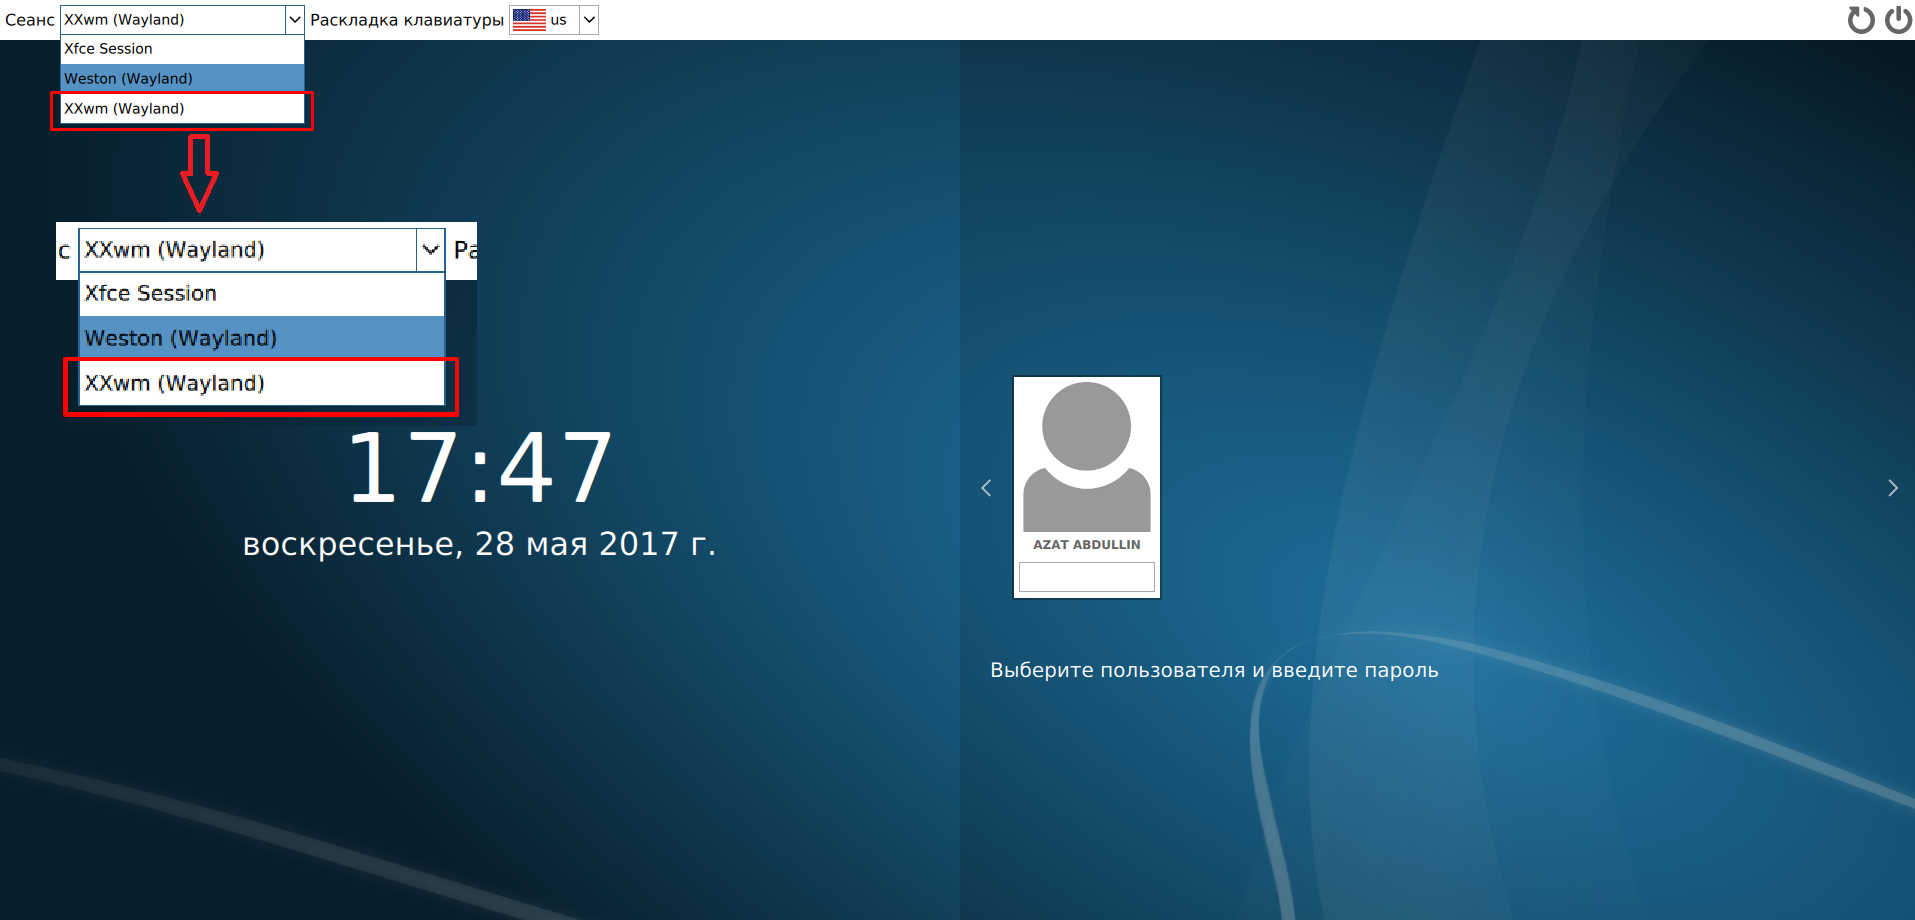
\includegraphics[width=\linewidth]{sddm}}
\caption{Пример загрузки ОМ через экранный менеджер}
\label{fig:sddm}
\end{figure}